% !Mode:: "TeX:UTF-8"
\documentclass{article}
\usepackage[UTF8,zihao=-4]{ctex}                     % 支持中文显示
\usepackage{graphicx}                       % 支持插图处理
% 支持版面尺寸设置
\usepackage{titlesec}                       % 控制标题的宏包
\usepackage{titletoc}                       % 控制目录的宏包
\usepackage{fancyhdr}                       % fancyhdr宏包 支持页眉和页脚的相关定义
\usepackage{color}                          % 支持彩色
\usepackage{amsmath}                        % AMSLaTeX宏包 用来排出更加漂亮的公式
\usepackage{amssymb}                        % 数学符号生成命令
\usepackage[below]{placeins}                %允许上一个section的浮动图形出现在下一个section的开始部分,还提供\FloatBarrier命令,使所有未处理的浮动图形立即被处理
\usepackage{flafter}                        % 使得所有浮动体不能被放置在其浮动环境之前,以免浮动体在引述它的文本之前出现.
\usepackage{multirow}                       % 使用Multirow宏包,使得表格可以合并多个row格
\usepackage{booktabs}                       % 表格,横的粗线;\specialrule{1pt}{0pt}{0pt}
\usepackage{longtable}                      % 支持跨页的表格。
\usepackage{tabularx}                       % 自动设置表格的列宽
\usepackage{subfigure}                      % 支持子图 %centerlast 设置最后一行是否居中
\usepackage[subfigure]{ccaption}            % 支持子图的中文标题
\usepackage[sort&compress,numbers]{natbib}  % 支持引用缩写的宏包
\usepackage{enumitem}                       % 使用enumitem宏包,改变列表项的格式
\usepackage{calc}                           % 长度可以用+ - * / 进行计算
\usepackage{txfonts}                        % 字体宏包
\usepackage{bm}                             % 处理数学公式中的黑斜体的宏包
\usepackage[amsmath,thmmarks,hyperref]{ntheorem}  % 定理类环境宏包,其中 amsmath 选项用来兼容 AMS LaTeX 的宏包
%如果您的pdf制作中文书签有乱码使用如下命令,就可以解决了
\usepackage{hyperref}
%%%%%%%%%%%%%%算法环境%%%%%%%%%%%%%%
\usepackage{listings}
\usepackage{xcolor}
\definecolor{dkgreen}{rgb}{0,0.6,0}
\definecolor{gray}{rgb}{0.5,0.5,0.5}
\definecolor{mauve}{rgb}{0.58,0,0.82}
\lstset{
	backgroundcolor=\color{gray!5},
	basicstyle={\linespread{1.1}\footnotesize\ttfamily},
	breakatwhitespace=true,
	breaklines=true,
	commentstyle=\color{dkgreen},
	frame=single,
	frameshape={RYRYNYYYY}{yny}{yny}{RYRYNYYYY},
	keywordstyle=\color{blue},
	language=Python,
	numbers=none,
	numberstyle=\tiny\color{gray},
	rulecolor=\color{gray!35},
	showstringspaces=false,
	stringstyle=\color{mauve},
	tabsize=4,
	aboveskip=3mm,
	belowskip=3mm,
	columns=flexible,
	framerule=1pt,
}
%%%%%%%%%%%%%%算法环境%%%%%%%%%%%%%%
%%%%%%%%%%%%去除目录红框%%%%%%%%%%%%
\hypersetup{
	colorlinks=true,
	linkcolor=black,
}
%%%%%%%%%%%%去除目录红框%%%%%%%%%%%%
%%%%%%%%%%%%%调整页边距%%%%%%%%%%%%%
\usepackage{geometry}
\geometry{a4paper,left=2cm,right=2cm,top=2cm,bottom=2cm}
%%%%%%%%%%%%%调整页边距%%%%%%%%%%%%%











\begin{document}

\title{图像处理作业——图像复原}
\author{刘坤鑫\thanks{3017218061 软件工程一班}}
\date{\today}
\maketitle
\begin{abstract}
	本文采用Python编程,主要调包skimage,以Lenna标准图像为研究对象,采用了7种噪声对其灰度图进行处理,高效地实现了课件中所有的10种滤波器,加上skimage自带的高斯模糊和均值滤波器2种滤波器,产生共$10*12=120$张结果图,并进行了简要的对比分析。
\end{abstract}

\section{Lenna标准测试图像}

\begin{figure}[ht]
	\centering
	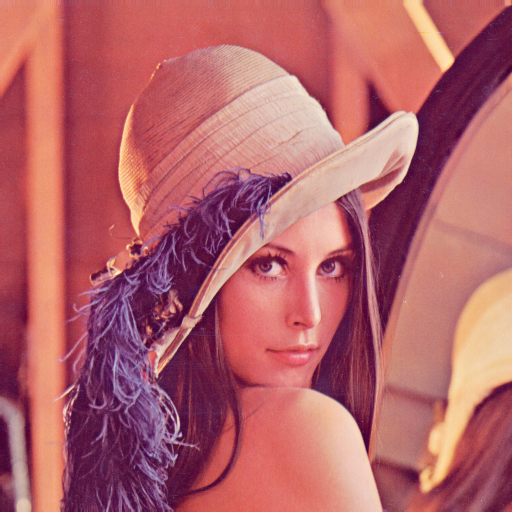
\includegraphics[width=0.6\linewidth]{fig/Lena.png}
	\caption{Lenna}
	\label{fig:Lenna}
\end{figure}

如图\ref{fig:Lenna}所示,Lenna或Lena是自1973年以来在图像处理领域广泛使用的标准测试图像的名称。可在WiKi上获取512x512的标准处理图像以及原图\footnote{https://en.wikipedia.org/wiki/Lenna}。

\section{添加噪声}

利用python的包skimage进行加噪处理,共包含以下噪声:

\begin{lstlisting}[title={skimage.util.random\_noise中mode参数设置}]
mode = [
	'gaussian',
	'localvar',
	'poisson',
	'salt',
	'pepper',
	's&p',
	'speckle',
]
\end{lstlisting}

\begin{figure}[ht]
	\centering
	\subfigure[Lenna with gaussian noise]{
		
\includegraphics[width=7cm]{fig/gaussian.png}
		%\caption{fig1}
	}
	\quad
	\subfigure[Lenna with salt and pepper noise]{
		
\includegraphics[width=7cm]{fig/s&p.png}
	}
	\caption{Lenna with noise}
	\label{fig:noise}
\end{figure}

如图\ref{fig:noise}为部分加噪效果图。为方便处理,加噪前已经将原图转为灰度图。完整结果参见github\footnote{https://github.com/qq734628996/image\_processing/tree/master/homework2/img}。

\section{滤波器实现}

本文实现了课件中所有的共10种滤波器,并添加了skimage自带的2种滤波器作为对比:

\begin{lstlisting}[title={12种滤波器对应函数名}]
filters = [
	arithmeticMeanFilter,
	geometricMeanFilter,
	harmonicMeanFilter,
	inverseHarmonicMeanFilter,
	medianFilter,
	maximumFilter,
	minimumFilter,
	medianRangeFilterFilter,
	improvedAlphaMeanFilter,
	AdaptiveMedianFilter,
	skimageGaussian,
	skimageMedian,
]
\end{lstlisting}

在实现非自适应滤波器时,考虑到所有滤波器都是共同的操作——卷积。理论上,卷积操作已经有了很好的计算优化。为了简单起见,又不失为充分考虑Python语言特性,并利用numpy进行计算加速。封装函数如下:

\begin{lstlisting}[title={填充边界,存储掩模}]
def _paddingFilling(image, m=3, n=3):
    up, down = image[0], image[-1]
    for i in range(m // 2):
        image = np.vstack([up, image, down])
    left, right = image[:, [0]], image[:, [-1]]
    for i in range(n // 2):
        image = np.hstack([left, image, right])
    return image

def _imageSpliting(image, m=3, n=3):
    height, width = image.shape
    oldImage = _paddingFilling(image, m, n)
    oldImages = []
    for i in range(m):
        for j in range(n):
            oldImages.append(oldImage[i:i + height, j:j + width])
    oldImages = np.asarray(oldImages)
    return oldImages
\end{lstlisting}

上述代码实现了图像的边界处理,并且保存每个像素对应的掩码块。有了上述代码,非自适应滤波器的实现变得统一而简单。例如算术平均滤波器的实现如下:

\begin{lstlisting}[title={算术平均滤波器}]
def arithmeticMeanFilter(image, m=3, n=3):
    oldImages = _imageSpliting(image, m=m, n=n)
    newImage = np.mean(oldImages, axis=0)
    return newImage
\end{lstlisting}

在笔者i5的笔记本上运行512x512的Lenna图片,只需要0.01s。

剩下非自适应滤波器实现几乎同理,除了要注意不要出现除以0的情况,均无太大区别,且运行速度不差。对于自适应中值滤波器,网上代码大都冗长而低效,本文在此给出一个简介而高效的Python实现:

\begin{lstlisting}[title={自适应中值滤波器}]
def AdaptiveMedianFilter(image, SMax=7):
    height, width = image.shape
    newImage = image.copy()
    for i in range(height):
        for j in range(width):
            filterSize = 3
            z = image[i][j]
            while(filterSize <= SMax):
                S = filterSize//2
                tmp = image[max(0, i-S): i+S+1, max(0, j-S): j+S+1].reshape(-1)
                tmp.sort()
                zMin = tmp[0]
                zMax = tmp[-1]
                zMed = tmp[len(tmp)//2]
                if(zMin < zMed and zMed < zMax):
                    if(z == zMin or z == zMax):
                        newImage[i][j] = zMed
                    break
                else:
                    filterSize += 2
    return newImage
\end{lstlisting}

完整代码参见github\footnote{https://github.com/qq734628996/image\_processing/tree/master/homework2/filter.py}

\section{结果展示}

\begin{figure}[ht]
	\centering
	\subfigure[算术平均滤波器]{
		
\includegraphics[width=7cm]{fig/gaussian_arithmeticMeanFilter.png}
		%\caption{fig1}
	}
	\quad
	\subfigure[中值滤波器]{
		
\includegraphics[width=7cm]{fig/gaussian_medianFilter.png}
	}
	\\
	\subfigure[逆谐波均值滤波器]{
		
\includegraphics[width=7cm]{fig/gaussian_inverseHarmonicMeanFilter.png}
	}
	\quad
	\subfigure[自适应中值滤波器]{
		
\includegraphics[width=7cm]{fig/gaussian_AdaptiveMedianFilter.png}
	}
	\caption{不同滤波器复原后的高斯噪声Lenna图}
	\label{fig:gao-filter}
\end{figure}

如图\ref{fig:gao-filter}只展示了四种效果良好的滤波器,其余滤波器效果均不理想。对于高斯噪声,图像很难再复原到原图像的模样。其中,算术平均滤波器效果和逆谐波均值滤波器效果近似,中值滤波器减少了图像模糊,但留下了比较多的噪声。自适应均值滤波器笔者认为在细节上做的最好,在尽可能保留细节的情况下,尽可能地减少噪声。

\begin{figure}[ht]
	\centering
	\subfigure[改进阿尔法均值滤波器]{
		
\includegraphics[width=7cm]{fig/s&p_improvedAlphaMeanFilter.png}
		%\caption{fig1}
	}
	\quad
	\subfigure[中值滤波器]{
		
\includegraphics[width=7cm]{fig/s&p_medianFilter.png}
	}
	\\
	\subfigure[自适应中值滤波器]{
		
\includegraphics[width=7cm]{fig/s&p_AdaptiveMedianFilter.png}
	}
	\quad
	\subfigure[skimage自带的中值滤波器]{
		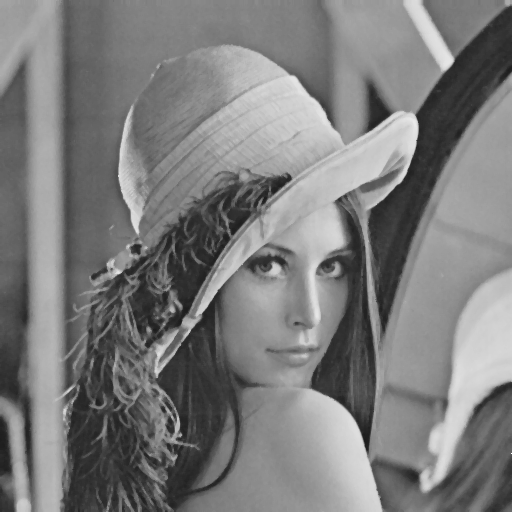
\includegraphics[width=7cm]{fig/s&p_skimageMedian.png}
	}
	\caption{不同滤波器复原后的椒盐噪声Lenna图}
	\label{fig:sp-filter}
\end{figure}

如图\ref{fig:sp-filter}只展示了四种效果良好的滤波器,其余滤波器效果均不理想。其中,改进阿尔法均值滤波器很大程度上去除了了椒盐噪声,中值滤波器几乎去除了所有的椒盐噪声,自适应中值滤波器不仅去除了所有的椒盐噪声,还保留了图像细节(如帽子纹路),skimage自带的中值滤波器和本文实现的中值滤波器略有区别,但整体效果几乎一样。

完整结果参见github\footnote{https://github.com/qq734628996/image\_processing/tree/master/homework2/img}。

\clearpage
\section*{附录}

完整Python代码如下:

\begin{lstlisting}[title={filter.py}]
#!/usr/bin/env python
# -*- coding:utf-8 -*-

from skimage import io
from PIL import Image
import skimage
import skimage.filters
import numpy as np
import matplotlib.pyplot as plt
import functools
import time
import os


def _paddingFilling(image, m=3, n=3):
    up, down = image[0], image[-1]
    for i in range(m // 2):
        image = np.vstack([up, image, down])
    left, right = image[:, [0]], image[:, [-1]]
    for i in range(n // 2):
        image = np.hstack([left, image, right])
    return image


def _imageSpliting(image, m=3, n=3):
    height, width = image.shape
    oldImage = _paddingFilling(image, m, n)
    oldImages = []
    for i in range(m):
        for j in range(n):
            oldImages.append(oldImage[i:i + height, j:j + width])
    oldImages = np.asarray(oldImages)
    return oldImages


def arithmeticMeanFilter(image, m=3, n=3):
    oldImages = _imageSpliting(image, m=m, n=n)
    newImage = np.mean(oldImages, axis=0)
    return newImage


def geometricMeanFilter(image, m=3, n=3):
    oldImages = _imageSpliting(np.log(image + 1e-6), m=m, n=n)
    newImage = np.exp(np.mean(oldImages, axis=0))
    return newImage


def harmonicMeanFilter(image, m=3, n=3):
    oldImages = _imageSpliting(1 / (image + 1e-6), m=m, n=n)
    newImage = (1 / np.mean(oldImages, axis=0))
    return newImage


def inverseHarmonicMeanFilter(image, m=3, n=3, Q=1):
    oldImages1 = _imageSpliting((image + 1e-6) ** (Q + 1), m=m, n=n)
    oldImages2 = _imageSpliting((image + 1e-6) ** Q, m=m, n=n)
    return np.sum(oldImages1, axis=0) / np.sum(oldImages2, axis=0)


def medianFilter(image, m=3, n=3):
    oldImages = _imageSpliting(image, m=m, n=n)
    newImage = np.median(oldImages, axis=0)
    return newImage


def maximumFilter(image, m=3, n=3):
    oldImages = _imageSpliting(image, m=m, n=n)
    newImage = np.max(oldImages, axis=0)
    return newImage


def minimumFilter(image, m=3, n=3):
    oldImages = _imageSpliting(image, m=m, n=n)
    newImage = np.min(oldImages, axis=0)
    return newImage


def medianRangeFilterFilter(image, m=3, n=3):
    oldImages = _imageSpliting(image, m=m, n=n)
    newImage = (np.max(oldImages, axis=0) + np.min(oldImages, axis=0)) / 2
    return newImage


def improvedAlphaMeanFilter(image, m=3, n=3, d=2):
    d = d // 2
    oldImages = _imageSpliting(image, m=m, n=n)
    oldImages = np.sort(oldImages, axis=0)
    newImage = np.mean(oldImages[d:m * n - d], axis=0)
    return newImage


def AdaptiveMedianFilter(image, SMax=7):
    height, width = image.shape
    newImage = image.copy()
    for i in range(height):
        for j in range(width):
            filterSize = 3
            z = image[i][j]
            while(filterSize <= SMax):
                S = filterSize//2
                tmp = image[max(0, i-S): i+S+1, max(0, j-S): j+S+1].reshape(-1)
                tmp.sort()
                zMin = tmp[0]
                zMax = tmp[-1]
                zMed = tmp[len(tmp)//2]
                if(zMin < zMed and zMed < zMax):
                    if(z == zMin or z == zMax):
                        newImage[i][j] = zMed
                    break
                else:
                    filterSize += 2
    return newImage


def skimageGaussian(image, sigma=1):
    newImage = skimage.filters.gaussian(image, sigma=sigma)
    return newImage


def skimageMedian(image):
    newImage = skimage.filters.median(image)
    return newImage


def main():
    basePath = 'img'
    imagePath = os.path.join(basePath, 'lena512.bmp')
    image = io.imread(imagePath)
    mode = [
        'gaussian',
        'localvar',
        'poisson',
        'salt',
        'pepper',
        's&p',
        'speckle',
    ]
    filters = [
        arithmeticMeanFilter,
        geometricMeanFilter,
        harmonicMeanFilter,
        inverseHarmonicMeanFilter,
        medianFilter,
        maximumFilter,
        minimumFilter,
        medianRangeFilterFilter,
        improvedAlphaMeanFilter,
        AdaptiveMedianFilter,
        skimageGaussian,
        skimageMedian,
    ]
    for m in mode:
        print(m)
        path = os.path.join(basePath, m)
        if not os.path.exists(path):
            os.mkdir(path)
        imageNoise = skimage.util.random_noise(image, mode=m)
        savePath = os.path.join(path, '{}.png'.format(m))
        io.imsave(savePath, imageNoise)
        for f in filters:
            savePath = os.path.join(path, '{}_{}.png'.format(m, f.__name__))
            io.imsave(savePath, f(imageNoise))


if __name__ == "__main__":
    main()

\end{lstlisting}

























\end{document}

